\section{数据集制作流程}

不同源光学影像超分数据集制作后期流程如图\ref{fig:0101}所示:

\begin{figure}[htbp]
    \centering
    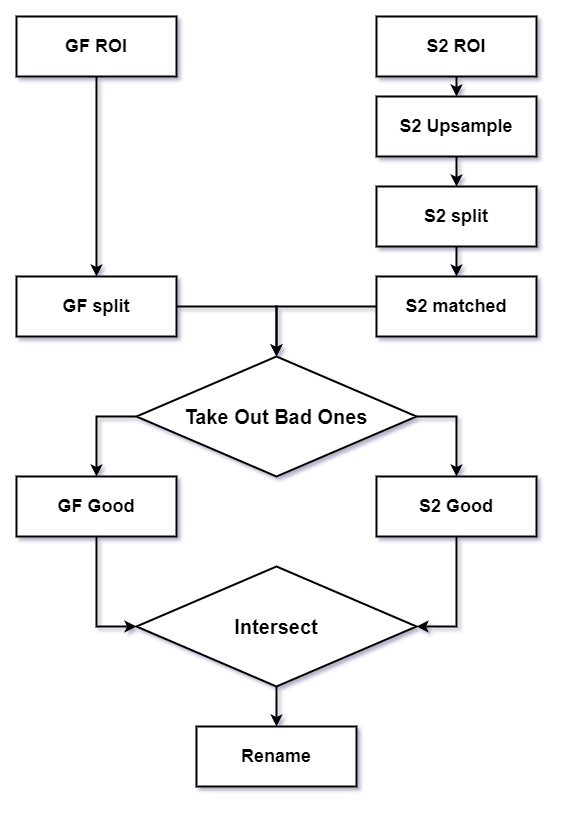
\includegraphics[height=0.7\textheight]{pic/chap01.png}
    \caption{整体流程图}
    \label{fig:0101}
\end{figure}

在ENVI中对原始遥感影像进行预处理, 影像精匹配, 裁剪后分别得到高分影像和哨兵影像的感兴趣区域, 即空间匹配效果较好的影像大块(ENVI格式, 遥感影像). 将其转换为png图片后, 此基础上, 进行数据集的制作. 哨兵影像分辨率为10m $\times$ 10m, 高分影像分辨率为 2m $\times$ 2m. 为了适配模型最高4倍的超分, 需要对哨兵影像进行上采用至分辨率8m $\times$ 8m. 

首先分别对影像进行批量裁剪, 其目的是增加高低分辨率影像对. 由于两幅影像范围相同, 分辨率不同, 因此为了得到空间匹配的高分辨率和低分辨率影像对, 两幅影像需按照相同比例裁剪. 裁剪之后, 为了保证色调一致, 需进行直方图匹配, 本次数据集制作使用的2021年IEEE一篇论文代码, 链接为~\href{https://github.com/hahnec/color-matcher}{ColorMatcher}. 之后人工分别高分影像和哨兵影像云雾遮挡严重和水田差异明显的影像进行剔除, 对剔除后的高低分辨率求交集, 得到质量较好的高低分辨率, 之后根据DIV2K数据集对其重命名, 便可用于训练.

完成并整合了python脚本, 通过脚本1完成上采样, 裁剪, 直方图匹配, 脚本2完成人工挑选后数据的交集和重命名. 